\section{Block-Algebra (BA)}\label{sec:block-algebra}

\kasten{%
\subsubsection*{Block Algebra overview}
\begin{calcfeatures}
\feature{calculus identifier}{block-algebra,ba}
\feature{calculus parameter}{none}
\feature{arity}{binary}
\feature{entity tape}{axis-aligned boxes, $(x_{\mathrm{min}}, y_{\mathrm{min}}, x_{\mathrm{max}}, y_{\mathrm{max}})$}
\feature{description}{describes spatial arrangement of boxes by independently projecting to x- and y-axis intervals and applying Allen's Interval Algebra (see \secref{sec:allen}) to both dimensions (see \figref{fig:block-algebra})}
\feature{base relations}{relations $r\_s$, whereby $r,s$ are Allen relations which yields $13\cdot13 = 169$ base relations}
\lastfeature{references}{\citet{guesgen:89,DBLP:journals/logcom/BalbianiCC02}}
\end{calcfeatures}
}

\begin{figure}[b]
\centerline{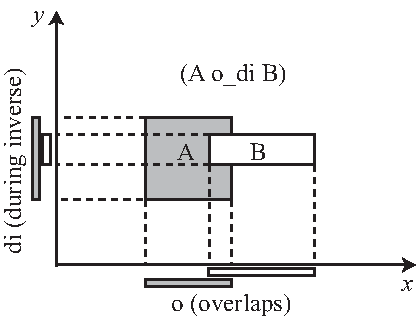
\includegraphics{block-algebra}}
\caption{\label{fig:block-algebra}Example relation o\_di in the block algebra}
\end{figure}